\documentclass[12pt]{article}
\usepackage{setspace, graphicx, fullpage, amssymb, amsmath, epsfig, natbib, array, multirow}
\usepackage[bookmarks = false, hidelinks]{hyperref}
\usepackage{amsfonts, bm}
\usepackage{dcolumn}
\usepackage{subfigure, float}
\usepackage[margin=1in]{geometry}
\usepackage{verbatim}
\usepackage{url}
\usepackage{enumerate}
\usepackage{morefloats}
\usepackage[skip = 2pt]{caption}
\usepackage[flushleft]{threeparttable}
\usepackage[T1]{fontenc}
\usepackage{libertine}
\usepackage{scrextend}
\usepackage{setspace}
\usepackage{fancyhdr}
\usepackage{enumitem}
\usepackage{natbib}

\newcommand\fnote[1]{\captionsetup{font=normalsize}\caption*{#1}}

\setlist{nolistsep,noitemsep}
\setlength{\footnotesep}{1.2\baselineskip}
\deffootnote[.2in]{0in}{0em}{\normalsize\thefootnotemark.\enskip}
\newcolumntype{.}{D{.}{.}{-1}}
\newcolumntype{d}[1]{D{.}{.}{#1}}

\makeatother

\def\citeapos#1{\citeauthor{#1}'s (\citeyear{#1})} % possessive citation



\begin{document}

\bibliographystyle{apsr}

\title{Party Calls and Reelection in the U.S. Senate\thanks{
We would like to thank Andrew Podob for reviewing a draft of this paper.
ADD FURTHER ACKNOWLEDGEMENTS?}
}

\author{
  Ethan Hershberger\thanks{
    \small Ohio State University
  }\quad
  William Minozzi$^\dagger$\quad
  Craig Volden\thanks{
    \small University of Virginia
  }\\
}

\date{\today}

\maketitle

\begin{center}

\vspace{.1in}
Word Count: XXXX
\end{center}
\vspace{.25in}

\begin{abstract}
\singlespacing
\noindent
\cite{Minozzi:2013} advance the idea that a substantial portion of partisan
voting activity in Congress is a simple call to unity that is especially easily embraced by ideological extremists.  If correct, their findings should extend from the House to the Senate, despite Senate leaders lacking many of the sticks and carrots found in the House.  We adapt the theory and measurement of party calls to the Senate.  In so doing, we find that both the House and the Senate have relied heavily (and increasingly) on party calls over the past four decades.  In the Senate in particular, the lens of party calls opens new opportunities for scholars to explore partisan legislative behavior.  We take advantage of one such opportunity to show how electoral concerns limit Senators' responsiveness to party calls.
\end{abstract}

\clearpage
\setcounter{page}{1}

\doublespacing

\noindent When scholars think of partisan influence in legislative voting they often conceive of pressure exerted on fence-sitting legislators to win them over to the party leaders' preferred position.  Given such a conception, party leaders in the Senate are thought to be less influential than their House counterparts because they possess fewer tools and opportunities to exert pressure.\footnote{\doublespacing\normalsize Yet, recent work has shown significant party effects in the Senate
% (e.g., Gailmard and Jenkins 2007; Monroe, Roberts, and Rohde 2008; Patty 2008; Volden and Bergman 2006)
\citep[e.g.,][]{Gailmard:2007, Monroe:2008, Patty:2008, Volden:2006}.
} In contrast with a pressure-based approach to understanding parties, \cite{Minozzi:2013} offer a theory of party calls. They suggest that, on many issues, unity among party members serves broad partisan ends, such as brand development
\citep[e.g.,][]{Snyder:2002}, apart from attempts to win closely contested votes on legislation. As a result, leaders' attempts to call party members to vote together will be more influential on extremists (who benefit from a coherent brand) than on cross-pressured moderates. Minozzi and Volden identify party-call votes and find enhanced responsiveness to them among extremists in the U.S. House.

We argue that the logic of party calls extends to the U.S. Senate, even in the absence of strong tools to exert control over the institution's individualistic members. We adapt the Minozzi and Volden approach to the Senate, and find strong evidence of party calls uniting party members, especially inducing ideological extremists to vote with the rest of the party, above and beyond their natural tendencies.

In addition to extending the examination of party calls to the Senate, we expand the time period of examination from the Volden and Minozzi study to include the 93$^{\text{rd}}$ through the 112$^{\text{th}}$ Congresses (1973-2012) for both the House and the Senate. Consistent with other evidence of partisan polarization across this era, we see a steady rise in the use of party calls over time across both chambers and regardless of Democrat or Republican control. Finally, we argue that extending the study of party calls to the Senate opens numerous opportunities for important new scholarship. Illustrating one such possibility, we show that Senators up for reelection are significantly less responsive to party calls, consistent with bucking the party when it is out of line with voters in their home states.

\subsection*{Party Calls in the Senate}

To explore party calls, \cite{Minozzi:2013} use a two-step process, first dividing floor votes into ``party-free votes" and ``party calls," and then examining which legislators are most responsive to party calls beyond their baseline partisan support on party-free votes. Identifying party calls is itself a tricky process, requiring researchers to identify a strong party-based voting pattern apart from that produced by ideological differences alone. We mimic the Minozzi and Volden iterative approach that produces the list of party-call votes and simultaneously generates party-free ideological ideal points for each legislator.\footnote{\doublespacing\normalsize As detailed in the Supplemental Appendix A, minor modifications were made to adapt this method to the Senate and to reduce computational burdens.}

As detailed in the Supplemental Appendix, the party calls identified through this process broadly reflect properties expected of partisan votes. For example, party calls tend to drive a further wedge between Democrats and Republicans who are already initially separated on ideological grounds. Moreover, party calls are more likely to occur among close votes than lopsided votes, perhaps because the close votes offer greater opportunity for parties to differentiate themselves.  In total, these patterns lend confidence that our classification of party-call votes is meaningful in capturing broad and consistent underlying behavior.

Figure~\ref{fig-party-calls-over-time} illustrates the percentage of party calls among all votes in the House and Senate. Across both chambers, the use of party calls has been steadily increasing over time.\footnote{\doublespacing\normalsize Because of the different threshold for identifying party calls across chambers, as well as their different membership sizes, direct House-Senate comparisons in the proportion of party-call votes would be inappropriate.} It is possible that parties are calling more because partisan ideological alignment has made party calls more effective, or because parties need members to rally more to get their agendas through a heavily gridlocked Congress. We believe that the underlying cause of this trend merits further investigation, but initially take it as evidence of much discussed increased partisanship and polarization in recent decades (e.g.,  \cite{Aldrich:2000, Lee:2009, Lee:2016, Theriault:2013, Smith:2014}). This trend holds regardless of which party is in the majority in the chamber.

\begin{figure}[p]
\centering
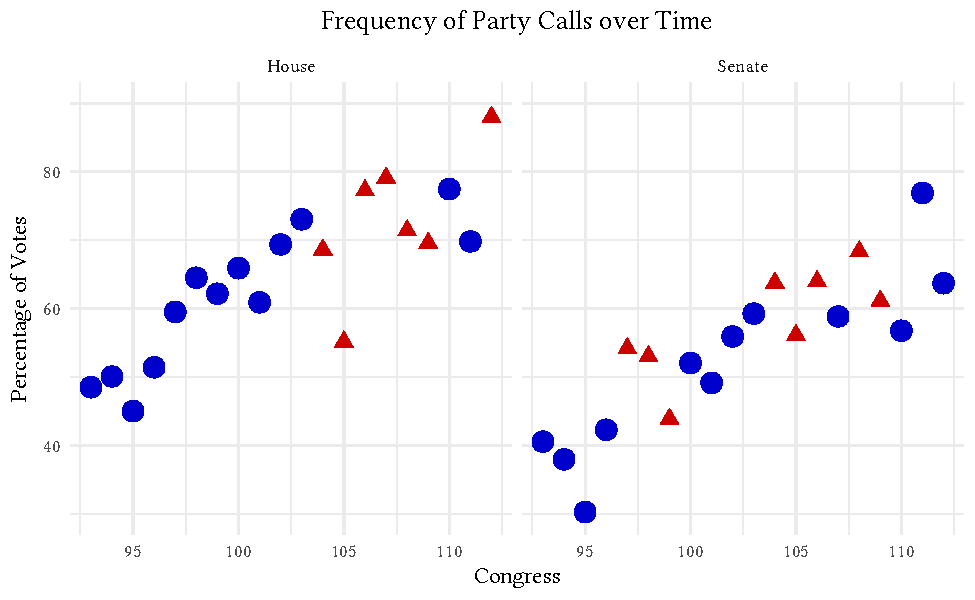
\includegraphics[width = \textwidth]{party_call_percent_both.pdf}
\caption{Party calls as a percentage of all votes, 1973-2012.
This figure shows the percentage of votes classified as party calls per Congress in each chamber. Blue circles denote Democrat-majority Congresses while Red triangles denote Republican-majority Congresses.
\label{fig-party-calls-over-time}}
\end{figure}

Fundamental to the theory of party calls is the idea that substantial partisan activity in Congress is designed to align members who might otherwise wander away from the party for idiosyncratic reasons, instead of solely winning close votes. As such, those most responsive to party calls are the extremists who tend to benefit from coherent party positions, rather than cross-pressured, fence-sitting moderates. To test this ``responsive extremists hypothesis," we run a series of OLS regressions, with a dependent variable measuring each legislator's percent support for the party position on party-call votes. We cluster the observations by legislator to account for possible dependence over time. Table~\ref{tab-responsiveness-regressions} shows that the responsive extremists hypothesis holds up well in the extended period over which we examine the House, and nearly as prominently in the Senate.


\begin{table}[!htbp]
\centering
\begin{threeparttable}
\caption{Models of Responsiveness to Party Calls, 1973-2012}
\label{tab-responsiveness-regressions}
\singlespacing
\begin{tabular}{l c c c }
\hline
& House & \multicolumn{2}{c}{Senate} \\
\hline
Ideological Extremism             & $7.75^{***}$  & $6.29^{***}$  & $6.24^{***}$  \\
                                  & $(0.13)$      & $(0.25)$      & $(0.25)$      \\
Baseline Rate of Voting with Party& $0.57^{***}$  & $0.73^{***}$  & $0.74^{***}$  \\
                                  & $(0.01)$      & $(0.02)$      & $(0.02)$      \\
Up for Reelection                 &               &               & $-0.94^{**}$  \\
                                  &               &               & $(0.36)$      \\
Vote Share                        & $-0.01$       & $0.03$        & $0.03$        \\
                                  & $(0.01)$      & $(0.02)$      & $(0.02)$      \\
Pres. Vote Share                  & $0.03^{**}$   & $0.10^{***}$  & $0.10^{***}$  \\
                                  & $(0.01)$      & $(0.02)$      & $(0.02)$      \\
Party Leader                      & $1.81^{***}$  & $1.65^{**}$   & $1.64^{**}$   \\
                                  & $(0.50)$      & $(0.54)$      & $(0.54)$      \\
Committee Chair                   & $4.98^{***}$  & $2.09^{***}$  & $2.06^{***}$  \\
                                  & $(0.46)$      & $(0.45)$      & $(0.45)$      \\
Power Committee                   & $2.76^{***}$  & $-0.66$       & $-0.66$       \\
                                  & $(0.23)$      & $(0.62)$      & $(0.62)$      \\
Best Committee                    & $-0.17^{***}$ & $0.15$        & $0.15$        \\
                                  & $(0.02)$      & $(0.10)$      & $(0.10)$      \\
Female                            & $1.17^{***}$  & $2.05^{**}$   & $2.03^{**}$   \\
                                  & $(0.32)$      & $(0.64)$      & $(0.64)$      \\
African American                  & $1.90^{***}$  & $-4.56$       & $-4.67$       \\
                                  & $(0.43)$      & $(2.49)$      & $(2.49)$      \\
Latino                            & $3.27^{***}$  & $5.60^{**}$   & $5.66^{**}$   \\
                                  & $(0.51)$      & $(1.82)$      & $(1.82)$      \\
South                             & $-0.89^{***}$ & $0.62$        & $0.61$        \\
                                  & $(0.21)$      & $(0.36)$      & $(0.36)$      \\
Seniority                         & $-0.05$       & $0.01$        & $0.01$        \\
                                  & $(0.03)$      & $(0.04)$      & $(0.04)$      \\
Freshman                          & $0.78^{**}$   & $1.08$        & $0.81$        \\
                                  & $(0.29)$      & $(0.56)$      & $(0.57)$      \\
Intercept                         & $31.78^{***}$ & $11.71^{***}$ & $11.94^{***}$ \\
                                  & $(1.30)$      & $(2.27)$      & $(2.27)$      \\
\hline
R$^2$                             & 0.46          & 0.63          & 0.63          \\
Adj. R$^2$                        & 0.46          & 0.63          & 0.63          \\
Num. obs.                         & 8544          & 1993          & 1993          \\
RMSE                              & 8.44          & 6.99          & 6.98          \\
\hline
% \multicolumn{4}{l}{\scriptsize{$^{***}p<0.001$, $^{**}p<0.01$, $^*p<0.05$, two-tailed tests.}}
\end{tabular}
% \fnote{\textit{Note}: Ordinary Least Squares models reported with dependent variable capturing percent of party-call votes in which the legislator votes with the majority of his or her party. Data are from the 93$^{rd}$-112$^{th}$ Congresses, with observations clustered by legislator.}
\begin{tablenotes}
   \item
   Ordinary Least Squares models reported with dependent variable capturing percent of party-call votes in which the legislator votes with the majority of his or her party. Data are from the 93$^{\text{rd}}$-112$^{\text{th}}$ Congresses, with observations clustered by legislator.
   $^{***}p<0.001$, $^{**}p<0.01$, $^*p<0.05$
 \end{tablenotes}
\end{threeparttable}
\end{table}

We include all of the control variables used by \cite{Minozzi:2013}, thus accounting for the \textit{Baseline Rate of Voting with Party} on the party-free votes.\footnote{\doublespacing\normalsize Descriptions and summary statistics for all control variables are given in the Supplemental Appendix C.} Although some House-Senate differences emerge, such as for Southerners or those on power committees, many broad patterns are consistent across institutions.\footnote{\doublespacing\normalsize Given the small size of the Senate, most members are included in the top committees, likely limiting the variance that allowed patterns to be discerned in the House based on committee assignments.} For example, positive coefficients show \textit{Party Leaders} and \textit{Committee Chairs} to be understandably highly responsive to party calls.

As shown by the coefficients on the \textit{Ideological Extremism} variable, and in strong support of the theory of party calls, each one-standard-deviation increase in ideological extremism is associated with a nearly eight-percentage-point increase in voting with their party in the House, and more than a six-percentage-point increase in the Senate.\footnote{\doublespacing\normalsize These effect sizes are consistent with those uncovered by \cite{Minozzi:2013} in the House between 1973 and 2006.} This party alignment extends above and beyond the baseline level of support of the member's party on non-party-call votes.

As detailed in the Supplemental Appendix, the pattern of ideological extremists being more responsive to party calls than moderates holds for both Democrats and Republicans, for both those in the majority party and those in the minority party. This robust support is illustrated in Figure~\ref{fig-extremism-responsiveness} based on separate regressions for each party in each Congress, a very tough test of the responsive extremists hypothesis, especially given the small membership of the Senate. In the House, ideological extremism takes a positive coefficient for all but four cases, and in the Senate for all but two. Further, in the House, all positive coefficients are statistically significant; in the Senate, 29 of the 38 positive coefficients are statistically significant, while only one negative coefficient is. These results add confidence to the aggregate findings above.

\begin{figure}[!htbp]
\centering
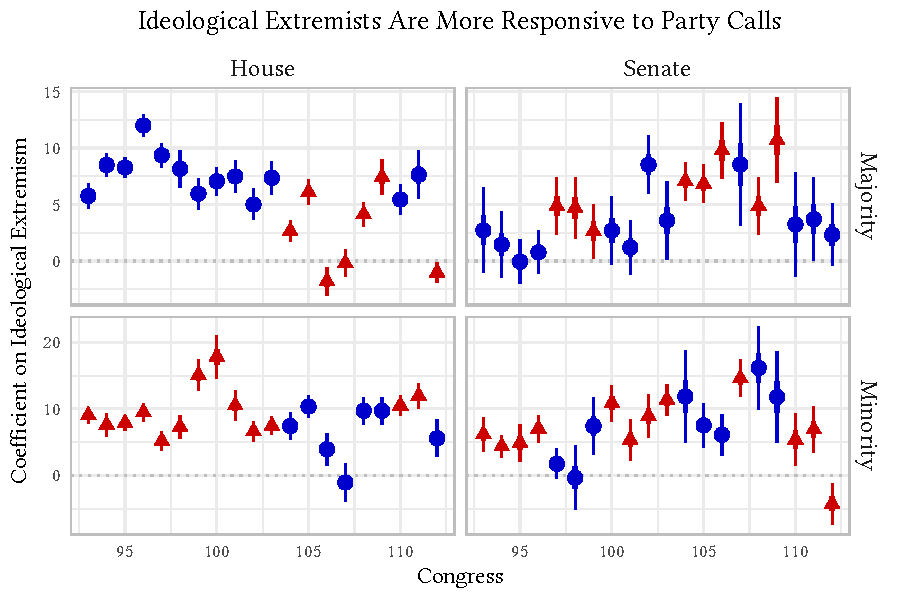
\includegraphics{both-chambers-figure2.pdf}
\caption{Extremists are responsive to party calls in both chambers.
This coefficient plot is produced by the same formula shown in the House and Senate regression table with results decomposed for the majority and minority parties in each of the 93$^{\text{rd}}$-112$^{\text{th}}$ Congresses (1973-2012). Coefficients shown are for the effect of ideological extremism on party-call votes, with both 50\% and 95\% confidence intervals shown.
\label{fig-extremism-responsiveness}}

% \fnote{\textit{Note}: This coefficient plot is produced by the same formula shown in the House and Senate regression table with results decomposed for the majority and minority parties in each of the 93$^{\text{rd}}$-112$^{\text{th}}$ Congresses (1973-2012). Coefficients shown are for the effect of ideological extremism on party-call votes, with both 50\% and 95\% confidence intervals shown.}
\end{figure}

In sum, the results reported here offer a coherent portrait of party calls in both chambers of the U.S. Congress. Party-call votes are widespread and increasing over the past four decades. They divide Democrats from Republicans, but especially draw ideologically extreme party members toward a unified partisan position.

Beyond uncovering such a systematic and important partisan process in Congress, the party calls identified here offer the potential to significantly enhance scholarly exploration of parties in the Senate. New research based on party calls could contribute to a fuller understanding of partisan practices and norms spreading from the House to the Senate \citep[e.g.,][]{Theriault:2013}, of the role of partisanship in advancing and overcoming filibusters \citep[e.g.,][]{Wawro:2004}, and of electoral constraints on partisan behavior \citep[e.g.,][]{Levitt:1996}, to name a few opportunities.

To illustrate the usefulness of party calls, we here briefly tackle the last of these possibilities. Specifically, in the final column of Table~\ref{tab-responsiveness-regressions}, we include an indicator variable for whether a Senator is in her final Congress before reelection. We expect that Senators are more free to help develop a party brand, even in contrast to their constituents' preferences, when electoral threats are behind them than when the next election is imminent. Consistent with this hypothesis, Table~\ref{tab-responsiveness-regressions} shows about one percentage point lower responsiveness to party calls among those facing reelection than among those in their first four years following an election, all else equal. In the next section, we explore this result more fully.

\subsection*{Reelection Limits Responsiveness to Party Calls}

We argue that Senators up for reelection will be more attuned to their electoral needs than to broad party interests. Put simply, they will use some party-call votes to aid their personal -- rather than the party -- brand
\citep[e.g.,][]{Canes-Wrone:2002, Carson:2010}.  Such a pattern was initially detected above.

As an alternate test, we here rely on same-state Senator pairs in which one Senator is up for reelection at the end of the Congress. These pairings are ideal because same-state Senators are elected by the same constituents, but not at the same time. This allows us to estimate a generalized difference-in-differences design. Apart from reelection, any additional differences between members from the same state should cancel each other out across Senators and over time, limiting the possibility of spuriously significant findings. Based on the logic above, we expect that the Senator up for reelection will be less responsive to party calls than her same-state Senate partner. In contrast, we expect no difference between the baseline rate of voting with the party absent party calls.

\begin{figure}[!htbp]
\centering

\includegraphics[width = 12cm]{senate_difference_estimates.pdf}

\caption{Senators up for reelection are less responsive to party calls.
This coefficient plot is produced by a paired differences model that uses same-state Senators as a natural pairing. Estimates shown are the difference in responsiveness to party calls and the baseline rate of voting with the party. Results are from OLS models, with 50\% and 95\% confidence intervals shown.
\label{fig-reelection-responsiveness}}
\end{figure}

Figure~\ref{fig-reelection-responsiveness} shows that member responsiveness to party calls declines, on average, about 1.5\% when they are up for reelection.\footnote{\doublespacing\normalsize In an alternative approach, we compare all three possibilities of same-state Senator pairs.  Comparing those up for reelection to those in their first Congress after election shows a similar effect to that in Figure~\ref{fig-reelection-responsiveness}.  Likewise, comparing those up for reelection to those in the middle two years of their six-year term reveals less responsiveness to party calls for those up for reelection.  In contrast, comparing same-state Senators, neither of whom are up for reelection, we find no difference in responsiveness.  Across all three cases, we find no differences in their rate of voting with the party on non-party-call votes, which acts as a placebo test.} However, their baseline rate of voting with the party is unchanged by electoral considerations. During the period of analysis, the average rate of responsiveness to party calls is 85\%. Across the XXX party-call votes in the average Senate, a Senator not up for reelection therefore averages XXX defection from her party.  In contrast, those up for reelection defect from party calls XXX times on average, about a ten percent increase.  Such deviations may limit the party's effectiveness in lawmaking and in developing a coherent brand.  But they offer the election-seeking Senator an opportunity to build her support and reputation back home.

\subsection*{Conclusion}

In this paper, we established that legislators respond to party calls in the Senate as they do in the House. In both chambers, party calls have become more prominent over the past forty years.  In line with expectations, when leaders issue party calls, legislators align with their party, with the greatest effect being among ideological extremists.

One especially noteworthy finding is therefore the nature of the relationship we uncover between party and ideology.  In contrast to \citeapos{Krehbiel:1993} view that partisanship is often merely a reflection of ideology, or \citeapos{Lee:2009} view that party extends well beyond ideology, we find party and ideology to be largely complementary but distinct.  When the party calls its members together, those who benefit the most -- typically ideological extremists -- respond most vigorously to the call.

We further showed the value of party calls as a tool for studying legislative behavior.  We found that reelection reduced member responsiveness to party calls.  Under electoral threat, constituent preferences are front and center in Senators' minds, and thus we hypothesized -- and found -- that members up for reelection are less responsive to the party. This finding shows one of the limits to the party-building efforts inherent in party calls.

\clearpage

\bibliography{senate}

\clearpage

\setcounter{table}{0}
\setcounter{footnote}{0}
\setcounter{figure}{0}
\setcounter{page}{0}

\refstepcounter{section}
\markright{Supplemental Appendices}

\begin{center}
\vspace*{1in}
{\Large Supplemental Appendices to\\}
{\LARGE Party Calls and Reelection in the U.S. Senate}
\end{center}
\vspace*{1in}

\thispagestyle{empty}

\setcounter{tocdepth}{1}
\setcounter{secnumdepth}{0}
\tableofcontents

\renewcommand\thetable{A\arabic{table}}
\renewcommand\thepage{A\arabic{page}}

\clearpage

\subsection*{Appendix A: Detailing the New Sorting Algorithm}
\addcontentsline{toc}{section}{\protect\numberline{}Detailing the New Sorting Algorithm}%

As in \citep{Minozzi:2013}, we use an algorithm to classify votes as ``party calls''---that is, whether votes are predicted by party membership even after controlling for ideology.  We classify the complement of votes as ``party free,'' and we use them to estimate ideal points absent party influence.  The classification algorithm is iterative.  In each iteration of the algorithm, ideal points are estimated based only on the votes which were classified as ``party free'' in the previous iteration.  All votes are then regressed on ideal points and party membership, and votes are re-categorized based on the explanatory power of party in these regressions.  To begin the process we need an initial classification, and so ideal points in the first iteration are estimated using lopsided votes (which have more than 65\% or less than 35\% of members of the chamber voting on the same side).  We then use a 15 iteration ``burn-in'' period for each Congress.  During this early period, many votes switch categories from iteration to iteration.  This number of switchers also declines rapidly in these early iterations.  After burn-in, the algorithm continues until either (1) the number of votes that switch classifications stops declining, or (2) until there are fewer than 5 votes that switch.  Once either condition is met, it continues for an additional 15 iterations.  Finally, we use the last five iterations to provide a final classification of votes. During these final iterations, any vote that does not switch is classified in its appropriate category.  Any vote which does switch is dropped from further analysis, on the basis that these votes could not be credibly classified.

Our algorithm departs from \citeapos{Minozzi:2013} in a few ways, most of them minor.  However, a key change was the use of the \textsf{binIRT} command from the \textsf{R} package \textsf{emIRT} \citep{Imai:2016} to estimate ideal points, replacing the \textsf{ideal} command from the \textsf{R} package \textsf{pscl} \citep{Jackman:2015} used by Minozzi \& Volden.  The \textsf{binIRT} function is considerably faster than \textsf{ideal}, and by using it, we were able to test a much wider variety of alternative specifications to the original algorithm.

The results of these alternative specifications culminated in a few alterations to the original algorithm.  Throughout, to ensure continuity of method, we vetted alternatives by re-estimating the results of \citep{Minozzi:2013} for the sake of comparison.  Those results are remarkably robust to the alternatives we explored.  Such robustness notwithstanding, we elected to make two minor changes.  First, the original classification algorithm used logistic regression to predict votes, meaning that party-line votes suffered from separation, which was resolved using a method for that purpose \citep{Zorn:2005}.  In this paper's classification method, we used linear models of roll call votes.  Second, the original algorithm classified votes as ``party calls'' if the $p$-value on the party indicator in a regression of a roll call vote was smaller than $0.01$.  However, the House roll call data features many more votes cast per roll call than the Senate, since the lower chamber is much larger.  As such, the threshold of $0.01$ eventuated in classifying very few Senate votes as party calls, essentially because of the smaller $n$.  We explored a variety of alternative $p$-value thresholds and settled on $0.05$, as it resulted in similar fractions of party calls across the two chambers.  Third, we also explored a variety of alternatives to the algorithm used here, but ultimately rejected them in order to maintain as much consistency with \citep{Minozzi:2013} as possible.  These included using random initial classifications of votes, adding a ``simulated annealing''-style heating and cooling schedule to categorizations, and alternative stopping rules.  We found that none of these alternatives significantly altered the results presented in the paper, and therefore elected to use an algorithm that closely matched the early effort.

Finally, with this algorithm in hand, we probed for differences in vote classifications between the two chambers.  First, we broke down votes by close/lopsideness and classification as party calls/party free.  Table~\ref{tab-close-lop} shows these comparisons for each chamber. In each panel, there is a notable, though far from perfect, correlation between close votes and party calls.  This correlation is higher in the House ($0.51$) than in the Senate ($0.45$), but the two are remarkably close.  We take this as prima facie evidence that the classification algorithm is at work on similar data-generating processes.

\begin{table}[H]
\centering
\begin{threeparttable}
\label{tab-close-lop}
\singlespacing
\caption{Party Calls and Close/Lopsided Votes}
\begin{tabular}{l cc cc}
\hline
&\multicolumn{2}{c}{\underline{House}}&\multicolumn{2}{c}{\underline{Senate}}\\
         & Party Call      & Party Free      & Party Call      & Party Free \\
\hline
Lopsided & $4245$ $(20\%)$ & $6123$ $(29\%)$ & $2063$ $(15\%)$ & $4876$ $(35\%)$ \\
Close    & $9308$ $(45\%)$ & $1090$ $(5\%)$  & $5233$ $(37\%)$ & $1851$ $(13\%)$ \\
\hline
\end{tabular}
\begin{tablenotes}
   \item
   The threshold for a vote to be lopsided was more than 65\% of members voting on the same side of a roll call vote.
 \end{tablenotes}
\end{threeparttable}
\end{table}

Next, we focus on whether the ``effects'' of party influence are working to exacerbate or to moderate those of ideology.
XXX
We find that the party call is not merely produced by a tradeoff of party and ideology explaining different votes.  They are on the same side approximately two-thirds of the time in the House and three-fifths of the time in the Senate.

\begin{table}[!htbp]
\centering
\begin{threeparttable}
\label{tab-sorting}
\singlespacing
\caption{Sorting Algorithm Coefficient Signs}
\begin{tabular}{l cc cc}
\hline
&\multicolumn{2}{c}{\underline{House}}&\multicolumn{2}{c}{\underline{Senate}}\\
& ($-$) Ideal & ($+$) Ideal & ($-$) Ideal & ($+$) Ideal \\
\hline
negative & 4581 & 2264 \\
  positive & 3224 & 4010 \\
($-$) Party & $8159$ $(38\%)$ & $3180$ $(15\%)$ & $4581$ $(33\%)$ & $2264$ $(16\%)$ \\
($+$) Party & $3739$ $(17\%)$ & $6405$ $(30\%)$ & $3224$ $(23\%)$ & $4010$ $(28\%)$ \\
\hline
\end{tabular}
\begin{tablenotes}
   \item
   The Party variable is an indicator for Republican and is positively correlated with ideal points.
 \end{tablenotes}
\end{threeparttable}
\end{table}

We found that the lowered number of both members and bills in the Senate required a few changes to the vote sorting method, however. Since $p$-values will necessarily be lower with fewer observations, we had to change the threshold for party calls to $p <$ 0.05 (from $p <$ 0.01). Next, since the ideal point algorithm uses a logistic regression, problems arose in vote sorting when we also tried to use another to sort vote type with this in the Senate. Neither change leads the sorting in the House to differ for the most part. We find that the sorting of close and lopsided votes by this method to be in line with Minozzi \& Volden's findings.


\clearpage

\subsection*{Appendix B: Methodology for Senate Reelection Section}
\addcontentsline{toc}{section}{\protect\numberline{}Methodology for Senate Reelection Section}%

To better test the role of reelection we use same-state senators as a natural pairing. These results were shown in Figure~\ref{fig-reelection-responsiveness} in the paper. The analyses we performed on these pairs were generalizations of the difference in differences design, in which the member not up for reelection had their rate of voting with the party on party calls and party free votes subtracted from that of the member who was up for reelection, as well as the difference between the response rate to party calls being subtracted from those of their same-state pairs.

As a further test, not shown in the paper, we estimated the effect of reelection and other variables with a fixed effects model. This produces substantively similar effects to those reported in the main paper. This allows us to decompose results by party. In doing so, we find results largely in line with those reported in the paper. Democrats show the least changes as reelection approaches, but for all categories the effect of reelection on party call responsiveness is negative and statistically significant.

\begin{table}[H]
\centering
\begin{threeparttable}
\label{tab-senate-fixeff}
\singlespacing
\small
\caption{Senate Fixed Effects Models}
\begin{tabular}{l c c c c c }
\hline
& All & Democrats & Republicans & Majority & Minority \\
\hline
Ideological Extremism  & $2.36^{***}$  & $2.88^{***}$ & $4.00^{***}$  & $1.94^{**}$   & $4.11^{***}$ \\
& $(0.48)$      & $(0.69)$     & $(0.75)$      & $(0.63)$      & $(0.88)$     \\
Baseline Rate of               & $0.35^{***}$  & $0.37^{***}$ & $0.25^{***}$  & $0.38^{***}$  & $0.22^{**}$  \\
\hspace{.7em}Voting with Party & $(0.03)$      & $(0.05)$     & $(0.05)$      & $(0.05)$      & $(0.07)$     \\
Up for Reelection     & $-1.01^{***}$ & $-0.55^{*}$  & $-1.55^{***}$ & $-1.03^{***}$ & $-0.91^{*}$  \\
& $(0.25)$      & $(0.27)$     & $(0.34)$      & $(0.28)$      & $(0.36)$     \\
Vote Share             & $-0.01$       & $0.03$       & $-0.05$       & $0.03$        & $-0.03$      \\
& $(0.02)$      & $(0.02)$     & $(0.03)$      & $(0.03)$      & $(0.03)$     \\
Pres. Vote Share       & $0.04$        & $0.27^{***}$ & $0.09$        & $0.32^{***}$  & $0.16^{**}$  \\
& $(0.02)$      & $(0.04)$     & $(0.05)$      & $(0.06)$      & $(0.06)$     \\
Freshman                & $1.31^{***}$  & $0.71$       & $0.98^{*}$    & $0.58$        & $0.64$       \\
& $(0.37)$      & $(0.48)$     & $(0.46)$      & $(0.44)$      & $(0.76)$     \\
Retiree                 & $0.52$        & $0.25$       & $0.88$        & $0.37$        & $0.60$       \\
& $(0.63)$      & $(0.83)$     & $(0.83)$      & $(0.96)$      & $(0.85)$     \\
Best Committee         & $0.18$        & $0.14$       & $0.11$        & $0.21$        & $0.32$       \\
& $(0.10)$      & $(0.12)$     & $(0.16)$      & $(0.16)$      & $(0.17)$     \\
Power Committee        & $-0.66$       & $-0.48$      & $-0.22$       & $-0.96$       & $-0.51$      \\
& $(0.61)$      & $(0.70)$     & $(0.98)$      & $(0.88)$      & $(0.93)$     \\
Party Leader                  & $1.27^{*}$    & $0.87$       & $1.46^{*}$    & $1.28$        & $1.12$       \\
& $(0.51)$      & $(0.47)$     & $(0.62)$      & $(0.71)$      & $(0.74)$     \\
Committee Chair                   & $2.93^{***}$  & $0.38$       & $0.65$        & $-0.36$       &              \\
& $(0.48)$      & $(0.64)$     & $(0.71)$      & $(0.56)$      &              \\
\hline
Num. obs.               & 1993          & 1042         & 951           & 1100          & 893          \\
R$^2$      & 0.87          & 0.89         & 0.91          & 0.91          & 0.93         \\
Adj. R$^2$ & 0.85          & 0.87         & 0.88          & 0.88          & 0.90         \\
\hline
% \multicolumn{6}{l}{{$^{***}p<0.001$, $^{**}p<0.01$, $^*p<0.05$}}
\end{tabular}
\begin{tablenotes}
   \item
   $^{***}p<0.001$, $^{**}p<0.01$, $^*p<0.05$
 \end{tablenotes}
\end{threeparttable}
\end{table}

\clearpage

\subsection*{Appendix C: Summary Statistics}
\addcontentsline{toc}{section}{\protect\numberline{}Summary Statistics}%

Here we give descriptions of report summary tables of the variables used in our paper. Members are grouped either as Democrats or Republicans, with independents being grouped with the party they caucus with in each chamber. The data are constructed with observations for members in each Congress they were present in. Values are according to member status in each Congress. Members who changed parties have multiple observations in the Congress which they did so to have observations for them in each. In each chamber, `Majority' is an indicator variable for if a members' party is in the majority during a Congress, which is used to divide results and summary statistics.\footnote{\doublespacing\normalsize For the purposes of analyses, Congress 107 in the Senate was given Democrats as the majority party and Republicans as the minority party since this was the case for most - but not all - of the Congress. This decision does not meaningfully impact results.}

Variables were acquired from the Legislative Effectiveness Project (or constructed with those data) with a few exceptions. Roll call data are from Keith Krehbiel's corrected roll call datasets, which were used to identify and measure response to party calls and party free votes. Committee data for the Senate and Congresses 110-112 in the House are from Charles Stewart's Congressional data page, with committee value ranks coming from Grimmer \& Stewart (2013). Committee data from Congresses 93-109 in the House are taken from the replication data for Minozzi \& Volden (2013). House vote share data were provided to us by Gary Jacobson, Senate vote share data are from Dave Leip's U.S. Election Atlas. Senate retiree data were collected from the Congressional Bioguides. Gingrich Senators were identified based on Theriault (2013).

`Party Free Ideal Point' is a member's ideal point (calculated by \verb|binIRT()| from the \verb|emIRT()| R package) based on party free votes only. It is centered at 0 with a standard deviation of 1, with a requirement that Democrats' values are on average lower (further left) than Republicans'. `Ideological Extremism' is this value with sign reversed for Democrats such that higher numbers represent more extreme members for both parties. `Party Call Response Rate' is the percent of times that a member voted with a majority of their party on party call votes. `Baseline Rate of Voting with Party' is the percent of times a member votes with a majority of their party on non-party call votes. The theoretical minimum for this variable is 0 and the maximum is 100.

\textit{Up for Reelection} is a Senate-specific variable, representing whether a member's election falls during a Congress. `Retiree' is an indicator variable for members who choose to leave office at or before the end of a Congress. `Vote Share' is calculated by the member's share of the vote relative to their nearest opponent.\footnote{\doublespacing\normalsize In the House, we report above or below average centered at 0 since unchallenged runs were coded as missing, to avoid selecting values for these. This decision had no impact on results.}  `Pres. Vote Share' in each chamber is an indication of Democrat or Republican (depending on who the member caucused with) presidential candidate 2-party vote share in the previous election based on the previous presidential election.  `Party Leader' is an indicator for if a member is in one of the positions identified as the congressional leadership (other than committee positions) in the Almanac of American Politics for a particular Congress. `Committee Chair' is an indicator for if a member chairs a committee in Congress. `Power Committee' represents a member being on one of the top four committees.  `Best Committee' takes a value based on the best committee a member was on, with values ranging from 0 (not on a committee) to the number of committees in the chamber (on the best committee). `Female' is an indicator variable for female legislators. `African American' is an indicator for African American legislators. `Latino' is an indicator for Hispanic and Latino legislators. `South' is an indicator for if a member represents a state or district from 13-state south. `Seniority' is a count variable of the number of consecutive Congresses a member has served in. `Freshman' is an indicator variable for the first Congress of a member previously not in Congress.



% Table created by stargazer v.5.2 by Marek Hlavac, Harvard University. E-mail: hlavac at fas.harvard.edu
% Date and time: Tue, May 16, 2017 - 11:58:48
\begin{table}[H]
\centering
\begin{threeparttable}
\singlespacing
\caption{Senate Summary Statistics}
\label{tab-senate-summary-stats}
\begin{tabular}{@{\extracolsep{5pt}}lcccc}
\\[-1.8ex]\hline
\hline \\[-1.8ex]
Variable & \multicolumn{1}{c}{Mean} & \multicolumn{1}{c}{St. Dev.} & \multicolumn{1}{c}{Min} & \multicolumn{1}{c}{Max} \\
\hline \\[-1.8ex]
Party Call Response Rate           & $85.5$  & $11.4$ & $8.8$ & $100$ \\
Party Free Ideal Point             & $0.00$  & $1.00$ & $-3.22$ & $3.40$ \\
Ideological Extremism              & $0.69$  & $0.72$ & $-1.63$ & $3.40$ \\
Baseline Rate of Voting with Party & $82.0$  & $8.2 $ & $45.1$ & $100$ \\
Up for Reelection                  & $0.33$  & $0.47$ & $0$ & $1$ \\
Retiree                            & $0.06$  & $0.24$ & $0$ & $1$ \\
Vote Share                         & $61.2$  & $9.9 $ & $50.0$ & $100$ \\
Pres. Vote Share                   & $52.1$  & $9.7 $ & $20.1$ & $78.0$ \\
Party Leader                       & $0.10$  & $0.30$ & $0$ & $1$ \\
Committee Chair                    & $0.18$  & $0.39$ & $0$ & $1$ \\
Power Committee                    & $0.73$  & $0.45$ & $0$ & $1$ \\
Best Committee                     & $12.3$  & $2.7 $ & $0$ & $15$ \\
Female                             & $0.07$  & $0.25$ & $0$ & $1$ \\
African American                   & $<0.01$ & $0.06$ & $0$ & $1$ \\
Latino                             & $0.01$  & $0.09$ & $0$ & $1$ \\
South                              & $0.26$  & $0.44$ & $0$ & $1$ \\
Seniority                          & $6.25$  & $4.62$ & $1$ & $26$ \\
Freshman                           & $0.11$  & $0.32$ & $0$ & $1$ \\
\hline \\[-1.8ex]
% \multicolumn{5}{l}{$N = 1,993$}
\end{tabular}
\begin{tablenotes}
   \item
   $N = 1,993$
 \end{tablenotes}
\end{threeparttable}
\end{table}

% Table created by stargazer v.5.2 by Marek Hlavac, Harvard University. E-mail: hlavac at fas.harvard.edu
% Date and time: Tue, May 16, 2017 - 11:58:51
%\begin{table}[H]
%\centering
%\singlespacing
%\caption{Senate Summary Statistics, Democrats}
%\label{}
%\begin{tabular}{@{\extracolsep{5pt}}lccccc}
%\\[-1.8ex]\hline
%\hline \\[-1.8ex]
%Statistic & \multicolumn{1}{c}{N} & \multicolumn{1}{c}{Mean} & \multicolumn{1}{c}{St. Dev.} & \multicolumn{1}{c}{Min} & \multicolumn{1}{c}{Max} \\
%\hline \\[-1.8ex]
%Party Free Ideal Point & 1,042 & $-$0.657 & 0.657 & $-$3.222 & 1.630 \\
%Ideological Extremism & 1,042 & 0.657 & 0.657 & $-$1.630 & 3.222 \\
%Party Call Response Rate & 1,042 & 85.776 & 10.886 & 8.777 & 100.000 \\
%Baseline Rate of Voting with Party & 1,042 & 83.760 & 7.862 & 45.106 & 100.000 \\
%Up for Reelection & 1,042 & 0.334 & 0.472 & 0 & 1 \\
%Retiree & 1,042 & 0.051 & 0.220 & 0 & 1 \\
%Vote Share & 1,042 & 0.619 & 0.102 & 0.500 & 1.000 \\
%Pres. Vote Share & 1,042 & 0.484 & 0.093 & 0.201 & 0.730 \\
%Party Leader & 1,042 & 0.083 & 0.277 & 0 & 1 \\
%Committee Chair & 1,042 & 0.208 & 0.406 & 0 & 1 \\
%Power Committee & 1,042 & 0.729 & 0.445 & 0 & 1 \\
%Best Committee & 1,042 & 12.257 & 2.780 & 0 & 15 \\
%Female & 1,042 & 0.084 & 0.278 & 0 & 1 \\
%African American & 1,042 & 0.005 & 0.069 & 0 & 1 \\
%Latino & 1,042 & 0.008 & 0.087 & 0 & 1 \\
%South & 1,042 & 0.236 & 0.425 & 0 & 1 \\
%Seniority & 1,042 & 6.781 & 4.940 & 1 & 26 \\
%Freshman & 1,042 & 0.105 & 0.306 & 0 & 1 \\
%\hline \\[-1.8ex]
%\end{tabular}
%\end{table}

% Table created by stargazer v.5.2 by Marek Hlavac, Harvard University. E-mail: hlavac at fas.harvard.edu
% Date and time: Tue, May 16, 2017 - 11:58:53
%\begin{table}[H]
%\centering
%\singlespacing
%\caption{Senate Summary Statistics, Republicans}
%\label{}
%\begin{tabular}{@{\extracolsep{5pt}}lccccc}
%\\[-1.8ex]\hline
%\hline \\[-1.8ex]
%Statistic & \multicolumn{1}{c}{N} & \multicolumn{1}{c}{Mean} & \multicolumn{1}{c}{St. Dev.} & \multicolumn{1}{c}{Min} & \multicolumn{1}{c}{Max} \\
%\hline \\[-1.8ex]
%Party Free Ideal Point & 951 & 0.725 & 0.789 & $-$1.595 & 3.397 \\
%Party Call Response Rate & 951 & 85.180 & 12.011 & 33.232 & 100.000 \\
%Baseline Rate of Voting with Party & 951 & 80.144 & 8.073 & 50.070 & 100.000 \\
%Ideological Extremism & 951 & 0.725 & 0.789 & $-$1.595 & 3.397 \\
%Up for Reelection & 951 & 0.332 & 0.471 & 0 & 1 \\
%Retiree & 951 & 0.067 & 0.251 & 0 & 1 \\
%Vote Share & 951 & 0.605 & 0.094 & 0.500 & 1.000 \\
%Pres. Vote Share & 951 & 0.562 & 0.085 & 0.310 & 0.780 \\
%Leader & 951 & 0.117 & 0.321 & 0 & 1 \\
%Committee Chair & 951 & 0.155 & 0.362 & 0 & 1 \\
%Power Committee & 951 & 0.723 & 0.448 & 0 & 1 \\
%Best Committee & 951 & 12.300 & 2.697 & 0 & 15 \\
%Female & 951 & 0.048 & 0.215 & 0 & 1 \\
%African American & 951 & 0.003 & 0.056 & 0 & 1 \\
%Latino & 951 & 0.007 & 0.086 & 0 & 1 \\
%South & 951 & 0.286 & 0.452 & 0 & 1 \\
%Seniority & 951 & 5.677 & 4.163 & 1 & 24 \\
%Freshman & 951 & 0.124 & 0.330 & 0 & 1 \\
%\hline \\[-1.8ex]
%\end{tabular}
%\end{table}

% Table created by stargazer v.5.2 by Marek Hlavac, Harvard University. E-mail: hlavac at fas.harvard.edu
% Date and time: Tue, May 16, 2017 - 11:58:55
%\begin{table}[H]
%\centering
%\singlespacing
%\caption{Senate Summary Statistics, Majority Party}
%\label{}
%\begin{tabular}{@{\extracolsep{5pt}}lccccc}
%\\[-1.8ex]\hline
%\hline \\[-1.8ex]
%Statistic & \multicolumn{1}{c}{N} & \multicolumn{1}{c}{Mean} & \multicolumn{1}{c}{St. Dev.} & \multicolumn{1}{c}{Min} & \multicolumn{1}{c}{Max} \\
%\hline \\[-1.8ex]
%Party Free Ideal Point & 1,052 & $-$0.071 & 0.918 & $-$1.966 & 2.866 \\
%Ideological Extremism & 1,052 & 0.614 & 0.687 & $-$1.630 & 2.866 \\
%Party Call Response Rate & 1,052 & 86.934 & 10.350 & 37.020 & 100.000 \\
%Baseeline Rate of Voting with Party & 1,052 & 83.089 & 8.216 & 45.106 & 100.000 \\
%Up for Reelection & 1,052 & 0.323 & 0.468 & 0 & 1 \\
%Retiree & 1,052 & 0.051 & 0.221 & 0 & 1 \\
%Vote Share & 1,052 & 0.614 & 0.100 & 0.500 & 1.000 \\
%Pres. Vote Share & 1,052 & 0.506 & 0.101 & 0.201 & 0.780 \\
%Party Leader & 1,052 & 0.096 & 0.295 & 0 & 1 \\
%Committee Chair & 1,052 & 0.329 & 0.470 & 0 & 1 \\
%Power Committee & 1,052 & 0.721 & 0.449 & 0 & 1 \\
%Best Committee & 1,052 & 12.270 & 2.755 & 0 & 15 \\
%Female & 1,052 & 0.065 & 0.246 & 0 & 1 \\
%African American & 1,052 & 0.002 & 0.044 & 0 & 1 \\
%Latino & 1,052 & 0.010 & 0.097 & 0 & 1 \\
%South & 1,052 & 0.267 & 0.443 & 0 & 1 \\
%Seniority & 1,052 & 6.089 & 4.618 & 1 & 26 \\
%Freshman & 1,052 & 0.129 & 0.336 & 0 & 1 \\
%
%\hline \\[-1.8ex]
%\end{tabular}
%\end{table}


% Table created by stargazer v.5.2 by Marek Hlavac, Harvard University. E-mail: hlavac at fas.harvard.edu
% Date and time: Tue, May 16, 2017 - 11:58:57
%\begin{table}[H]
%\centering
%\singlespacing
%\caption{Senate Summary Statistics, Minority Party }
%\label{}
%\begin{tabular}{@{\extracolsep{5pt}}lccccc}
%\\[-1.8ex]\hline
%\hline \\[-1.8ex]
%Statistic & \multicolumn{1}{c}{N} & \multicolumn{1}{c}{Mean} & \multicolumn{1}{c}{St. Dev.} & \multicolumn{1}{c}{Min} & \multicolumn{1}{c}{Max} \\
%\hline \\[-1.8ex]
%
%Party Free Ideal Point & 843 & 0.091 & 1.086 & $-$3.222 & 3.397 \\
%Ideological Extremism & 843 & 0.767 & 0.773 & $-$1.269 & 3.397 \\
%Party Call Response Rate & 843 & 83.138 & 12.372 & 8.777 & 100.000 \\
%Baseline Rate of Voting with Party & 843 & 80.354 & 8.068 & 50.070 & 100.000 \\
%Up for Reelection & 843 & 0.345 & 0.476 & 0 & 1 \\
%Retiree & 843 & 0.070 & 0.255 & 0 & 1 \\
%Vote Share & 843 & 0.611 & 0.098 & 0.500 & 1.000 \\
%Pres. Vote Share & 843 & 0.538 & 0.091 & 0.284 & 0.754 \\
%Party Leader & 843 & 0.102 & 0.303 & 0 & 1 \\
%Committee Chair & 843 & 0.000 & 0.000 & 0 & 0 \\
%Power Committee & 843 & 0.733 & 0.443 & 0 & 1 \\
%Best Committee & 843 & 12.284 & 2.711 & 0 & 15 \\
%Female & 843 & 0.064 & 0.245 & 0 & 1 \\
%African American & 843 & 0.007 & 0.084 & 0 & 1 \\
%Latino & 843 & 0.006 & 0.077 & 0 & 1 \\
%South & 843 & 0.250 & 0.433 & 0 & 1 \\
%Seniority & 843 & 6.409 & 4.545 & 1 & 24 \\
%Freshman & 843 & 0.096 & 0.295 & 0 & 1 \\
%\hline \\[-1.8ex]
%\end{tabular}
%\end{table}

% Table created by stargazer v.5.2 by Marek Hlavac, Harvard University. E-mail: hlavac at fas.harvard.edu
% Date and time: Tue, May 16, 2017 - 12:20:30
\begin{table}[H]
\centering
\begin{threeparttable}
\singlespacing
\caption{House Summary Statistics}
\label{tab-house-summary-stats}
\begin{tabular}{@{\extracolsep{5pt}}lcccc}
\\[-1.8ex]\hline
\hline \\[-1.8ex]
Variable & \multicolumn{1}{c}{Mean} & \multicolumn{1}{c}{St. Dev.} & \multicolumn{1}{c}{Min} & \multicolumn{1}{c}{Max} \\
\hline \\[-1.8ex]
Party Call Response Rate           & $85.8$ & $11.5$ & $8.0$ & $100$ \\
Party Free Ideal Point             & $0.00$ & $1.00$ & $-4.08$ & $9.35$ \\
Ideological Extremism              & $0.60$ & $0.80$ & $-4.32$ & $9.35$ \\
Baseline Rate of Voting With Party & $87.0$ & $ 7.5$ & $0$     & $100$ \\
Vote Share vs. Mean Vote Share     & $ 0.0$ & $ 9.2$ & $-15.7$ & $31.4$ \\
Pres. Vote Share                   & $56.6$ & $12.4$ & $16.3$  & $96.1$ \\
Party Leader                       & $0.04$ & $0.19$ & $0$     & $1$ \\
Committee Chair                    & $0.05$ & $0.22$ & $0$     & $1$ \\
Power Committee                    & $0.26$ & $0.44$ & $0$     & $1$ \\
Best Committee                     & $13.8$ & $ 6.4$ & $0$     & $22$ \\
Female                             & $0.09$ & $0.29$ & $0$     & $1$ \\
African American                   & $0.06$ & $0.24$ & $0$     & $1$ \\
Latino                             & $0.04$ & $0.18$ & $0$     & $1$ \\
South                              & $0.30$ & $0.46$ & $0$     & $1$ \\
Seniority                          & $5.33$ & $4.05$ & $1$     & $29$ \\
Freshman                           & $0.16$ & $0.36$ & $0$     & $1$ \\
% Democrat & 0.56 & 0.50 & 0 & 1 \\
% Majority & 0.57 & 0.50 & 0 & 1 \\
\hline \\[-1.8ex]
% \multicolumn{5}{l}{$N = 8,544$}
\end{tabular}
\begin{tablenotes}
   \item
   $N = 8,544$
 \end{tablenotes}
\end{threeparttable}
\end{table}

\clearpage

\subsection*{Other Tables and Figures}
\addcontentsline{toc}{section}{\protect\numberline{}Other Tables and Figures}%

Here we present results from regression models in the House and Senate which separately model by party or majority status. We expected that reelection would make members less responsive to the call of the party as they work to pivot to their districts when approaching reelection. We find that for all models categories that the sign is in the expected direction and that for all, save Democrats, it achieves statistical significance. Further, we should expect that those retiring are no longer beholden to their constituents and thus would not have this draw on their attention when the party calls. We find across all models that retirees' responsiveness to party calls takes a positive coefficient and for all, save Democrats, it is statistically significant.

We find that minority party women are substantially more responsive to party calls than their male counterparts in both chambers. Others have found that minority party women remain more focused on legislative agendas than their male counterparts \cite{Volden:2013}, and we take this finding as being in line with this account. While results for this are mixed, we find generally that increased same-party presidential vote share (an indicator of party strength in the district) increases responsiveness to party calls while increased personal vote share (an indicator of member popularity in the district) decreases responsiveness. However, this relationship does not present itself for Democrats. A number of factors complicate this relationship for Democrats, such as landslide presidential election losses and the presence of Southern Democrats early on who were more moderate than their copartisans.

\begin{table}[H]
\centering
\begin{threeparttable}
\label{tab-house-models}
\singlespacing
\small
\caption{House Responsiveness to Party Calls}
\begin{tabular}{l c c c c c }
\hline
& All & Democrats & Republicans & Majority & Minority \\
\hline
Ideological Extremism & $7.766^{***}$  & $8.350^{***}$  & $5.873^{***}$  & $6.713^{***}$  & $8.655^{***}$  \\
& $(0.130)$      & $(0.168)$      & $(0.207)$      & $(0.157)$      & $(0.201)$      \\
Baseline Rate of               & $0.575^{***}$  & $0.636^{***}$  & $0.414^{***}$  & $0.522^{***}$  & $0.632^{***}$  \\
\hspace{.7em}Voting With Party& $(0.012)$      & $(0.015)$      & $(0.020)$      & $(0.015)$      & $(0.020)$      \\
Vote Share            & $-0.007$       & $-0.058^{***}$ & $0.021$        & $-0.125^{***}$ & $-0.109^{***}$ \\
& $(0.012)$      & $(0.013)$      & $(0.022)$      & $(0.015)$      & $(0.019)$      \\
Pres. Vote Share      & $0.028^{**}$   & $0.099^{***}$  & $-0.098^{***}$ & $0.204^{***}$  & $0.185^{***}$  \\
& $(0.010)$      & $(0.011)$      & $(0.020)$      & $(0.012)$      & $(0.018)$      \\
Party Leader                 & $1.811^{***}$  & $1.972^{**}$   & $2.787^{***}$  & $2.627^{***}$  & $1.843^{**}$   \\
& $(0.497)$      & $(0.599)$      & $(0.761)$      & $(0.647)$      & $(0.653)$      \\
Committee Chair                  & $4.960^{***}$  & $2.552^{***}$  & $9.779^{***}$  & $1.964^{***}$  &                \\
& $(0.456)$      & $(0.498)$      & $(0.803)$      & $(0.444)$      &                \\
Power Committee                  & $2.756^{***}$  & $1.801^{***}$  & $2.931^{***}$  & $2.972^{***}$  & $1.135^{**}$   \\
& $(0.235)$      & $(0.275)$      & $(0.374)$      & $(0.269)$      & $(0.361)$      \\
Best Committee          & $-0.169^{***}$ & $-0.038^{*}$   & $-0.240^{***}$ & $-0.178^{***}$ & $-0.161^{***}$ \\
& $(0.016)$      & $(0.019)$      & $(0.025)$      & $(0.019)$      & $(0.023)$      \\
Female                 & $1.173^{***}$  & $0.615$        & $-0.078$       & $0.037$        & $2.228^{***}$  \\
& $(0.322)$      & $(0.353)$      & $(0.574)$      & $(0.404)$      & $(0.442)$      \\
African American                   & $1.835^{***}$  & $-0.470$       & $5.089$        & $-3.014^{***}$ & $3.402^{***}$  \\
& $(0.429)$      & $(0.441)$      & $(2.972)$      & $(0.536)$      & $(0.610)$      \\
Latino                 & $3.221^{***}$  & $1.711^{***}$  & $2.405^{*}$    & $2.453^{***}$  & $3.191^{***}$  \\
& $(0.507)$      & $(0.514)$      & $(1.153)$      & $(0.626)$      & $(0.705)$      \\
South                  & $-0.922^{***}$ & $-2.640^{***}$ & $3.610^{***}$  & $-2.180^{***}$ & $-0.667^{*}$   \\
& $(0.205)$      & $(0.276)$      & $(0.329)$      & $(0.244)$      & $(0.313)$      \\
Seniority              & $-0.053$       & $0.049$        & $-0.334^{***}$ & $0.011$        & $0.015$        \\
& $(0.028)$      & $(0.031)$      & $(0.050)$      & $(0.034)$      & $(0.041)$      \\
Freshman               & $0.834^{**}$   & $-0.058$       & $1.167^{*}$    & $0.346$        & $-0.456$       \\
& $(0.297)$      & $(0.356)$      & $(0.464)$      & $(0.348)$      & $(0.446)$      \\
Intercept            & $30.952^{***}$ & $21.282^{***}$ & $53.412^{***}$ & $30.032^{***}$ & $12.343^{***}$ \\
& $(1.217)$      & $(1.495)$      & $(2.174)$      & $(1.390)$      & $(2.106)$      \\
\hline
R$^2$                  & 0.460          & 0.631          & 0.303          & 0.564          & 0.478          \\
Adj. R$^2$             & 0.459          & 0.630          & 0.301          & 0.563          & 0.477          \\
Num. obs.              & 8544           & 4746           & 3798           & 4898           & 3646           \\
RMSE                   & 8.443          & 7.363          & 8.868          & 7.559          & 8.015          \\
\hline
\end{tabular}
% \multicolumn{6}{p{\wd0-2\tabcolsep-.25em}}}
% \fnote{Results are produced by OLS regressions for all members for the entire period in the first column, with additional analyses for all Democrats and Republicans as well as all members of the Majority and Minority party in Congresses 93-112 in the House of Representatives. Details on the variables are provided in Appendix C.
% $^{***}p<0.001$, $^{**}p<0.01$, $^*p<0.05$}
\begin{tablenotes}
   \item
   Results are produced by OLS regressions for all members for the entire period in the first column, with additional analyses for all Democrats and Republicans as well as all members of the Majority and Minority party in Congresses 93-112 in the House of Representatives. Details on the variables are provided in Appendix C.
$^{***}p<0.001$, $^{**}p<0.01$, $^*p<0.05$
 \end{tablenotes}
\end{threeparttable}
\end{table}

\begin{table}[H]
\centering
\begin{threeparttable}
\label{tab-senate-models}
\singlespacing
\small
\caption{Senate Responsiveness to Party Calls}
\small
\begin{tabular}{l c c c c c }
\hline
& All & Democrats & Republicans & Majority & Minority \\
\hline
Ideological Extremism & $6.242^{***}$  & $3.125^{***}$ & $7.799^{***}$  & $4.697^{***}$  & $7.963^{***}$ \\
& $(0.252)$      & $(0.410)$     & $(0.358)$      & $(0.315)$      & $(0.400)$     \\
Baseline Rate of               & $0.737^{***}$  & $0.760^{***}$ & $0.741^{***}$  & $0.703^{***}$  & $0.702^{***}$ \\
\hspace{.7em}Voting With Party& $(0.021)$      & $(0.030)$     & $(0.031)$      & $(0.025)$      & $(0.035)$     \\
Up for Reelection    & $-0.806^{*}$   & $-0.642$      & $-1.238^{*}$   & $-1.013^{*}$   & $-0.928$      \\
& $(0.361)$      & $(0.435)$     & $(0.551)$      & $(0.421)$      & $(0.616)$     \\
Retiree                & $1.403^{*}$    & $1.095$       & $1.173$        & $1.054$        & $1.650$       \\
& $(0.685)$      & $(0.888)$     & $(0.981)$      & $(0.843)$      & $(1.087)$     \\
Vote Share            & $0.029$        & $-0.053^{*}$  & $0.150^{***}$  & $-0.012$       & $0.077^{**}$  \\
& $(0.018)$      & $(0.022)$     & $(0.028)$      & $(0.021)$      & $(0.030)$     \\
Pres. Vote Share      & $0.097^{***}$  & $0.234^{***}$ & $-0.133^{***}$ & $0.182^{***}$  & $0.006$       \\
& $(0.018)$      & $(0.024)$     & $(0.031)$      & $(0.020)$      & $(0.032)$     \\
Party Leader                 & $1.607^{**}$   & $2.220^{**}$  & $0.908$        & $1.447^{*}$    & $1.923^{*}$   \\
& $(0.539)$      & $(0.712)$     & $(0.777)$      & $(0.660)$      & $(0.900)$     \\
Committee Chair                  & $2.109^{***}$  & $0.857$       & $3.621^{***}$  & $-0.025$       &               \\
& $(0.452)$      & $(0.543)$     & $(0.701)$      & $(0.517)$      &               \\
Power Committee       & $-0.672$       & $-0.835$      & $-0.335$       & $-0.019$       & $-1.475$      \\
& $(0.620)$      & $(0.771)$     & $(0.925)$      & $(0.719)$      & $(1.065)$     \\
Best Committee        & $0.160$        & $0.232$       & $0.009$        & $0.020$        & $0.374^{*}$   \\
& $(0.101)$      & $(0.124)$     & $(0.154)$      & $(0.118)$      & $(0.175)$     \\
Female                 & $2.046^{**}$   & $1.687^{*}$   & $0.475$        & $0.522$        & $4.268^{***}$ \\
& $(0.639)$      & $(0.730)$     & $(1.133)$      & $(0.758)$      & $(1.115)$     \\
African American                   & $-4.782$       & $-1.193$      & $-10.776^{*}$  & $1.522$        & $-5.536$      \\
& $(2.487)$      & $(2.789)$     & $(4.283)$      & $(4.183)$      & $(3.222)$     \\
Latino                 & $5.712^{**}$   & $1.805$       & $7.251^{**}$   & $4.778^{*}$    & $6.201$       \\
& $(1.816)$      & $(2.198)$     & $(2.782)$      & $(1.878)$      & $(3.510)$     \\
South                  & $0.611$        & $-1.701^{**}$ & $0.881$        & $0.053$        & $1.087$       \\
& $(0.362)$      & $(0.558)$     & $(0.579)$      & $(0.427)$      & $(0.623)$     \\
Seniority              & $0.001$        & $0.040$       & $-0.025$       & $0.077$        & $0.117$       \\
& $(0.044)$      & $(0.052)$     & $(0.072)$      & $(0.060)$      & $(0.070)$     \\
Freshman               & $0.887$        & $0.755$       & $0.427$        & $0.571$        & $1.086$       \\
& $(0.567)$      & $(0.710)$     & $(0.843)$      & $(0.633)$      & $(1.033)$     \\
Intercept            & $11.537^{***}$ & $9.432^{**}$  & $18.000^{***}$ & $16.344^{***}$ & $10.679^{**}$ \\
& $(2.274)$      & $(2.906)$     & $(3.491)$      & $(2.643)$      & $(4.013)$     \\
\hline
R$^2$                  & 0.632          & 0.689         & 0.641          & 0.684          & 0.614         \\
Adj. R$^2$             & 0.629          & 0.684         & 0.634          & 0.679          & 0.607         \\
Num. obs.              & 1993           & 1042          & 951            & 1052           & 843           \\
RMSE                   & 6.970          & 6.118         & 7.263          & 5.864          & 7.757         \\
\hline
\end{tabular}
% \fnote{Results are produced by OLS regressions for all members for the entire period in the first column, with additional analyses for all Democrats and Republicans as well as all members of the Majority and Minority party in Congresses 93-112 in the Senate. Details on the variables are provided in Appendix C.
% $^{***}p<0.001$, $^{**}p<0.01$, $^*p<0.05$}
\begin{tablenotes}
   \item
   Results are produced by OLS regressions for all members for the entire period in the first column, with additional analyses for all Democrats and Republicans as well as all members of the Majority and Minority party in Congresses 93-112 in the Senate. Details on the variables are provided in Appendix C.
$^{***}p<0.001$, $^{**}p<0.01$, $^*p<0.05$
 \end{tablenotes}
\end{threeparttable}
\end{table}

\end{document}
